\documentclass[border=8pt]{standalone}
\usepackage{tikz}
\usetikzlibrary{positioning,arrows.meta,calc,decorations.pathreplacing}
\usepackage[scaled=0.95]{helvet}
\renewcommand{\familydefault}{\sfdefault}
\definecolor{ink}{HTML}{1F2328}\definecolor{muted}{HTML}{57606A}
\definecolor{cS}{HTML}{8250DF}  % Stage 1 lead-lag selector
\definecolor{cEL}{HTML}{2A78D6} % Express Links
\definecolor{cFO}{HTML}{EB6834} % Forecast-only
\definecolor{cRA}{HTML}{1BAF7A} % random
\definecolor{fast}{HTML}{2DA44E}\definecolor{mid}{HTML}{D4A72C}\definecolor{slow}{HTML}{CF222E}
\hyphenpenalty=10000
% node positions: two clusters joined by one bridge (hL -- hR)
\def\nodelist{L1/0/0.5,L2/0/-0.5,L3/0.8/1.0,L4/0.8/0,L5/0.8/-1.0,L6/1.6/0.5,L7/1.6/-0.5,hL/2.35/0,hR/3.35/0,R1/4.1/0.5,R2/4.1/-0.5,R3/4.9/1.0,R4/4.9/0,R5/4.9/-1.0,R6/5.7/0.5,R7/5.7/-0.5}
\def\edgelist{L1/L3,L1/L4,L2/L4,L2/L5,L3/L6,L4/L6,L4/L7,L5/L7,L6/hL,L7/hL,hR/R1,hR/R2,R1/R3,R1/R4,R2/R4,R2/R5,R3/R6,R4/R6,R4/R7,R5/R7}
\def\rnsize{2.6mm}
% \road{prefix}{(shift)}{scale}{fill colour}
\newcommand{\road}[4]{%
  \begin{scope}[shift={#2}, scale=#3]
    \foreach \n/\x/\y in \nodelist {\coordinate (#1\n) at (\x,\y);}
    \foreach \a/\b in \edgelist {\draw[ink!45, line width=0.6pt] (#1\a)--(#1\b);}
    \draw[ink!70, line width=1.8pt] (#1hL)--(#1hR);
    \foreach \n/\x/\y in \nodelist {\node[circle, inner sep=0pt, minimum size=\rnsize, draw=ink!75, line width=0.45pt, fill=#4] at (#1\n) {};}
  \end{scope}}
\tikzset{newlink/.style={-{Stealth[length=2.2mm]}, line width=1.4pt, #1},
         arr/.style={-{Stealth[length=2.6mm]}, line width=1pt, draw=ink!65}}

\begin{document}
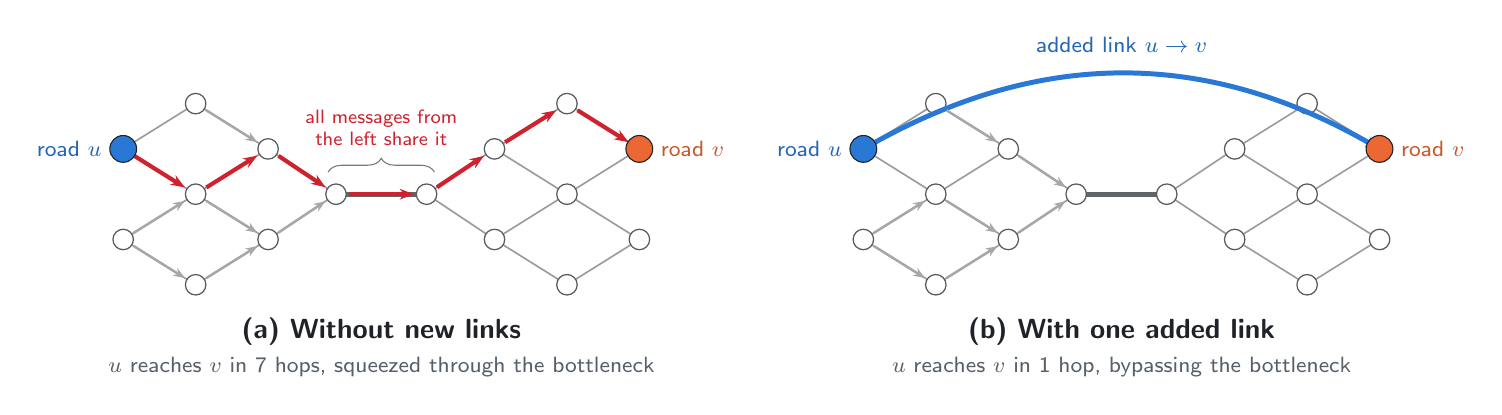
\begin{tikzpicture}[font=\small, color=ink,
  msg/.style={-{Stealth[length=1.8mm]}, line width=1.5pt, #1},
  crowd/.style={-{Stealth[length=1.5mm]}, line width=0.9pt, ink!40}]
% ---------- (a) without links
\road{a}{(0,0)}{1.15}{white}
\foreach \p/\q in {L1/L4,L4/L6,L6/hL,hL/hR,hR/R1,R1/R3,R3/R6}{\draw[msg=slow, shorten <=1.6mm, shorten >=1.6mm] (a\p) -- (a\q);}
\foreach \p/\q in {L3/L6,L2/L5,L5/L7,L7/hL,L2/L4,L4/L7}{\draw[crowd, shorten <=1.6mm, shorten >=1.6mm] (a\p) -- (a\q);}
\node[circle, fill=cEL, draw=ink, inner sep=0pt, minimum size=3.4mm] at (aL1) {};
\node[circle, fill=cFO, draw=ink, inner sep=0pt, minimum size=3.4mm] at (aR6) {};
\node[font=\footnotesize, text=cEL!85!black, anchor=east] at ($(aL1)+(-0.15,0)$) {road $u$};
\node[font=\footnotesize, text=cFO!85!black, anchor=west] at ($(aR6)+(0.15,0)$) {road $v$};
\draw[decorate, decoration={brace, amplitude=5pt}, ink!60] ($(ahL)+(-0.1,0.28)$) -- ($(ahR)+(0.1,0.28)$) node[midway, above=6pt, font=\scriptsize, text=slow, align=center] {all messages from\\the left share it};
\node[font=\bfseries, align=center] at (3.28,-1.75) {(a) Without new links};
\node[font=\footnotesize, text=muted, align=center] at (3.28,-2.2) {$u$ reaches $v$ in 7 hops, squeezed through the bottleneck};

% ---------- (b) with an express link
\begin{scope}[xshift=9.4cm]
\road{b}{(0,0)}{1.15}{white}
\draw[msg=cEL, line width=1.8pt] (bL1) to[bend left=30] (bR6);
\foreach \p/\q in {L3/L6,L2/L5,L5/L7,L7/hL,L2/L4,L4/L7,L6/hL}{\draw[crowd, shorten <=1.6mm, shorten >=1.6mm] (b\p) -- (b\q);}
\node[circle, fill=cEL, draw=ink, inner sep=0pt, minimum size=3.4mm] at (bL1) {};
\node[circle, fill=cFO, draw=ink, inner sep=0pt, minimum size=3.4mm] at (bR6) {};
\node[font=\footnotesize, text=cEL!85!black, anchor=east] at ($(bL1)+(-0.15,0)$) {road $u$};
\node[font=\footnotesize, text=cFO!85!black, anchor=west] at ($(bR6)+(0.15,0)$) {road $v$};
\node[font=\footnotesize, text=cEL!85!black] at (3.28,1.9) {added link $u\to v$};
\node[font=\bfseries, anchor=west] at (-0.6,1.75) {};
\node[font=\bfseries, align=center] at (3.28,-1.75) {(b) With one added link};
\node[font=\footnotesize, text=muted, align=center] at (3.28,-2.2) {$u$ reaches $v$ in 1 hop, bypassing the bottleneck};
\end{scope}
\node[font=\bfseries, anchor=west] at (-0.6,-2.0) {};
\end{tikzpicture}
\end{document}
